\documentclass[10pt]{article}
\usepackage[letterpaper,margin=0.7in,top=0.65in,bottom=0.7in]{geometry}
\usepackage[T1]{fontenc}
\usepackage{amsmath,amssymb}
\usepackage{txfonts}
\usepackage{booktabs,graphicx,caption,microtype,xcolor,tabularx,array,enumitem,multirow}
\usepackage[numbers,sort&compress]{natbib}
\usepackage[hidelinks]{hyperref}
\captionsetup{font=small,labelfont=bf,skip=3pt}
\setcounter{topnumber}{3}\setcounter{bottomnumber}{2}\setcounter{totalnumber}{4}
\renewcommand{\topfraction}{.95}\renewcommand{\bottomfraction}{.7}\renewcommand{\textfraction}{.05}\renewcommand{\floatpagefraction}{.85}
\setlength{\textfloatsep}{8pt}\setlength{\floatsep}{6pt}\setlength{\intextsep}{6pt}\setlength{\abovecaptionskip}{3pt}
\setlength{\parskip}{1pt}
\makeatletter\renewcommand\section{\@startsection{section}{1}{\z@}{-2.2ex \@plus -1ex \@minus -.2ex}{1.3ex \@plus.2ex}{\normalfont\large\bfseries}}
\renewcommand\subsection{\@startsection{subsection}{2}{\z@}{-1.8ex\@plus -1ex \@minus -.2ex}{1ex \@plus .2ex}{\normalfont\normalsize\bfseries}}
\renewcommand\paragraph{\@startsection{paragraph}{4}{\z@}{1.2ex \@plus1ex \@minus.2ex}{-1em}{\normalfont\normalsize\bfseries}}\makeatother
\setlength{\bibsep}{1.5pt}
\setlist{nosep,leftmargin=1.2em}
\graphicspath{{figures/}{../figures/}}
\newcommand{\osi}{\mathrm{OSI}}
\title{\vspace{-1.6em}\Large Forecasting Storm Outage Severity for Unseen Counties:\\Restoration Kinetics, Lead-Dependent Boosting, and a Selective State-Space Sequence Model\vspace{-0.3em}}
\author{\normalsize Team \textbf{Night Owls} --- Team lead: Pritam Kumar Deb\\
\small Kennesaw State University\\[-2pt]
\small INFORMS 2026 Data Mining Society Data Challenge --- Forecasting Infrastructure Resilience Under Extreme Weather\vspace{-1.2em}}
\date{}

\begin{document}
\maketitle

\begin{abstract}\small\noindent
The 2026 challenge asks for hourly Outage Severity Index (OSI) forecasts at four horizons for 63 counties whose outage record is withheld after March 13 23:00, using 239 fully observed counties for training. The four horizon columns are shifted views of a single 144-hour trajectory issued from one fixed origin. We forecast that trajectory with two views of the same causal information. The first is a nested stack of two gradient-boosting members on 209 features: a \emph{kinetics} member that predicts the residual from a first-order restoration prior, $\osi_{\mathrm{cut}}\,2^{-\ell/H}$, with half-life $H\approx13$\,h estimated inside each fit, and a \emph{direct} member that predicts the OSI level. A delayed-onset member, trained only on counties still out or still rising at the cutoff, is worse at every horizon and is not in the stack. The second view is a small bidirectional selective state-space sequence model, four seeds, with the same stratified early-stopping holdout in cross-validation and in the final fit. The submitted file is an equal half of that two-tree stack and the sequence model. A lead-bucket mix, refit with each fold held out, scores $0.01061/0.00964/0.00803/0.00710$; its paired county-bootstrap intervals against the half all include zero, so the file is the half, at $0.01062/0.00967/0.00805/0.00710$ for $t{+}1/6/24/48$\,h, 51/47/29/25\% below the hourly climatology. One county, Forest County, PA, still holds 28\% of the squared error. Neighbor features use Census internal points, which the weather notes list as optional static enrichment. The stack runs in about three minutes and the sequence model in about 59 minutes on one CPU thread.
\end{abstract}

\section{Problem structure}\label{sec:problem}
The data package provides 216 hourly rows (March 11--19, 2026) for 302 counties in IN, OH, PA and WV, with 23 weather fields for every hour (2.5-km URMA analyses \citep{depondeca2011} for wind and temperature, ERA5 reanalysis \citep{hersbach2020} for the rest) and the outage state ($P_t$, $N_t$, $D_t$, $R_t$, counts, lags) for the first 72 hours only in the 63 test counties. Two wind events crossed the region (Fig.~\ref{fig:event}): the first peaks on March 13--14, when 131 of the 239 training counties reach their maximum OSI (110 on March 13 alone), and a second, broader event on March 15--17 that is comparable in wind but much weaker in outages (mean training OSI 0.020 on March 14 versus 0.005 on March 16).

Three structural facts drive our design. \textbf{(i) One origin, not 144.} The template asks for $\osi_{t+h}$ for every hour $t$ of March 14--19, but no outage information becomes available after the cutoff, so every entry is a forecast from the same information set and the four columns are shifted copies of one trajectory $S_c(j)$, $j=0,\dots,143$, where the forecast hour $j$ counts hours after March 14 00:00 ($j+1$ hours after the cutoff): the $t{+}h$ column at origin $j$ equals $S_c(j{+}h)$. Consequently the four RMSEs score \emph{nested windows} of the same trajectory (bottom of Fig.~\ref{fig:event}); the $t{+}48$\,h column only scores hours from March 16 00:00 onward and never sees the first-wave restoration. Predicting one trajectory per county and filling the columns by shifting it guarantees cross-horizon consistency and never imputes the withheld window, which the rules forbid. \textbf{(ii) Scored lead times range from $h{+}1$ to 144 hours after the cutoff.} No new observed outages can update a forecast after that origin. This does not preclude time-series models: SARIMAX can use future weather as exogenous inputs, as in the 2025 challenge study \citep{ye2025sarimax}, but a per-county model fitted to a test county's 72 observed hours must estimate that county's weather response from a single storm onset. We instead pool counties to learn weather-dependent trajectories (we do not evaluate SARIMAX here or claim that it cannot represent a second wave). Persistence of the cutoff value is a weak baseline (RMSE 0.063--0.069, worse than predicting zero) because so many counties sit near their peak at the cutoff: the task is a cross-sectional regression of trajectories on cutoff state and known weather. \textbf{(iii) The metric is dominated by a few counties and by the first day.} OSI targets are zero-inflated (42\% of scored $t{+}1$\,h cells are exactly zero; median 0.0001, maximum 0.545) and, because the loss is pooled squared error, ten counties carry 65--75\% of the target energy $\sum y^2$ and March 14 alone carries 78\% of it in the $t{+}1$\,h window. A model is therefore judged mostly on how well it renders first-wave restoration in severely hit counties---a different regime from the hurricane-outage literature, which predicts the \emph{onset} of damage from forecast winds \citep{guikema2014,fatima2024}.

\begin{figure}[tb]\centering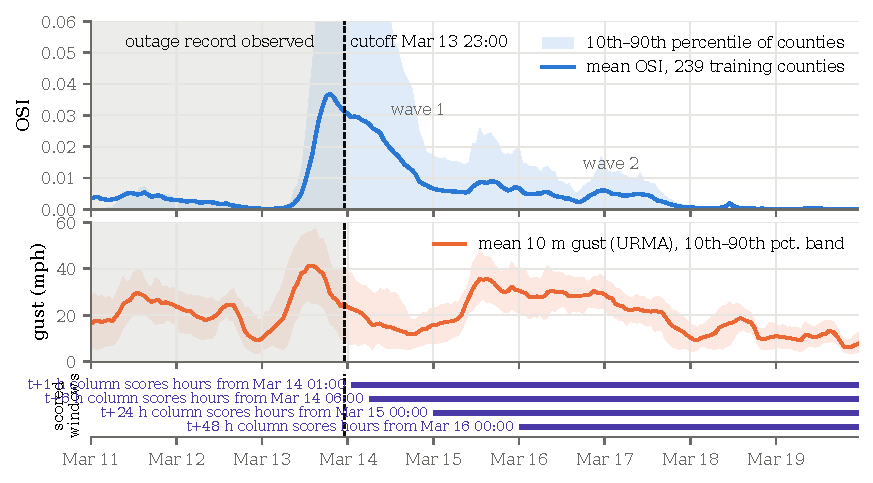
\includegraphics[width=.58\linewidth]{fig1_event_structure}
\caption{Event structure in the training counties (mean and 10th--90th percentile band). The shaded region is the only period with outage data in the test counties. Bottom: the hours scored by each submission column; all four are views of one trajectory issued at the cutoff.}\label{fig:event}\end{figure}

\section{Data handling and causal feature construction}\label{sec:data}
\paragraph{Validation.} Both files are checked for unique county-hour keys, complete 216-hour grids, disjoint county sets and, in the training file, equality of every stored target with the shifted OSI. OSI is reconstructed in the observed window as $\osi_t=\max(0,\,0.40P_t+0.35N_t+0.25D_t-0.10R_t)$ (the test file carries no \texttt{osi} or \texttt{osi\_lag} columns); on the training file this reproduces the stored values to $5\times10^{-5}$.

\paragraph{Information boundary.} For every county, the outage record is sliced to timestamps $\le$ March 13 23:00 \emph{before} any outage-derived quantity is computed; the centred-smoothed $N_t$ and $R_t$ at the cutoff hour are organiser-supplied values that the methodology document explicitly permits. Weather is used at any hour, past or future, as the rules allow. The training file also contains three undocumented per-county constants computed over the whole event (\texttt{peak\_pct}, \texttt{peak\_customers}, \texttt{time\_to\_restore\_h}), plus \texttt{severity\_tier}; none is a feature, and \texttt{severity\_tier} and state only stratify cross-validation folds. A mutation test, run on every execution, overwrites every post-cutoff outage field and every whole-event column, on the county being featurised and on the train-plus-test neighbour context, and asserts that the feature tensor is bitwise unchanged.

\paragraph{Features.} Each county yields a panel of $144\times209$ features indexed by lead $\ell=1,\dots,144$ hours after the cutoff. The families are (a) \emph{cutoff state and history}---levels, lags (0--48\,h), window means/maxima/standard deviations and changes of $P_t$ and reconstructed OSI over 3--72\,h, means of $N_t$, $R_t$, $D_t$, net inflow $N_t-R_t$ at the cutoff, hours since the observed peak; (b) \emph{exposure}---$\log(1+\text{median customers tracked})$; (c) \emph{lead coordinate}---$\ell$, $\log(1+\ell)$ and the cutoff OSI decayed with half-lives of 6/12/24/48\,h; (d) \emph{weather at the target hour}---all fields with wind direction encoded as $(\sin,\cos)$, temperatures in $^\circ$C and dew-point depression; (e) \emph{weather context}---trailing means and maxima, lagged and forward gusts, gust excess above 30/40/50\,mph, and gust$\times$soil-moisture and gust$\times$cutoff outage fraction \citep{cerrai2019}. Three neighbour features use other counties' \emph{cutoff} OSI only: an inverse-distance average, the nearest county's cutoff OSI, and that distance in kilometres. The coordinates are Census county internal points (\texttt{INTPTLAT}, \texttt{INTPTLONG}), shipped in \texttt{county\_centroids.csv}. The weather-variable notes list static geographic enrichment as optional; these points are static geography, not challenge outage fields. Icing hours, the 3\,h and 6\,h OSI slope, the unrepaired fraction, and the gust-excess ratio were built and then dropped: on the two-tree stack, removing each block one at a time lowered both the $t{+}24$\,h and the $t{+}48$\,h RMSE, while removing the neighbour block did not. Identifiers, names, timestamps, states, \texttt{severity\_tier} and the whole-event constants are never features.

\paragraph{Shape diagnostics.} We measured properties of the target and of its relation to the drivers on the training counties only (Table~\ref{tab:shape}; \texttt{shape\_diagnostics.py} reproduces every number). Each row fixes one design decision in Section~\ref{sec:method}: the zeros are not a separate onset process, the cutoff state loses its predictive value between 24 and 48 hours, and the wind response is strongly convex.

\begin{table}[tb]\centering\scriptsize
\caption{Shape diagnostics on the 239 training counties and the decision each fixes. Target statistics use the scored $t{+}1$\,h window; the mean--variance slope uses out-of-fold residuals of the boosting stack.}\label{tab:shape}
\begin{tabular}{@{}p{2.5cm}p{7.6cm}p{7.1cm}@{}}\toprule
Property & Statistic & Decision \\ \midrule
Availability at test time & Outage fields present for 100\% of hours before the cutoff, 0\% after; weather complete & One trajectory per county from one origin; no rolling models\\
Marginal distribution & 42\% exact zeros; positives span 3 decades ($\sigma_{\log_{10}}=0.88$); skewness 8.9, excess kurtosis 115; top 1\% of cells hold 72\% of $\sum y^2$ & Pooled RMSE is decided by a few severe counties; regularise, accept shrinkage of extremes\\
Origin of the zeros & 65\% of zero cells come from counties with cutoff OSI $\le0.005$ (29\% from counties at exactly zero); once a county with cutoff OSI $>0.005$ reaches zero, 66\% of its later hours stay zero & Zeros are ``not materially hit'' or ``restored'', driven by the same covariates as the level: no separate hurdle stage\\
Mean--variance relation & log--log slope of residual variance vs.\ predicted mean $=0.56$ for the stack, 0.90 for the submitted average (1: Poisson-like; 2: multiplicative) & Model the raw OSI with squared error; no log or Tweedie target\\
Temporal dependence & Within-county autocorrelation 0.98/0.79/0.29/0.05 at 1/6/24/48\,h; $R^2$ of the cutoff OSI for OSI at 1/24/48/96\,h after the cutoff $=0.99/0.78/0.09/0.00$ & A restoration prior owns the first day, weather owns days 3--6; hand-over weights by forecast hour with breaks after hours 12 and 48\\
Restoration kinetics & 74 counties with $\osi_{\mathrm{cut}}>0.02$: exponential fit, half-life median 13.1\,h (IQR 8--18\,h) & First-order prior with an estimated, not assumed, half-life\\
Response to the driver & Mean new-outage rate by gust bin 0--20/20--30/30--40/40--50/50+\,mph $=0.2/0.6/1.9/5.1/23\times10^{-3}$ & Convex, threshold-like: tree learners and gust-excess features; linear exogenous terms would be misspecified\\
Heterogeneity & State-level ICC of post-cutoff peaks = 0.082 (unequal-group one-way ANOVA) & Pool all counties in one model; no per-state or cluster models\\
Sample for the tail & 39 counties with post-cutoff peak $>0.1$; ten counties hold 65\% of $\sum y^2$ & Shallow trees, strong regularisation, county-level uncertainty statements\\
\bottomrule\end{tabular}\end{table}

\section{Method}\label{sec:method}
\subsection{A restoration-kinetics prior}
Restoration after a wind event is well described in the outage literature as a decay process whose rate depends on damage extent and crew capacity \citep{liu2007,nateghi2011}. Fig.~\ref{fig:kinetics}a shows the post-cutoff OSI of the 74 training counties with $\osi_{\mathrm{cut}}>0.02$, normalised by the cutoff value: after a short plateau most counties decay roughly exponentially, with a median $R^2$ of 0.86 for a one-parameter fit over the first 48 leads and per-county half-lives concentrated between 8 and 18\,h (Fig.~\ref{fig:kinetics}b). We therefore define a prior trajectory
\begin{equation}
\hat S^{\,0}_c(\ell)=\osi_{c,\mathrm{cut}}\;2^{-\ell/H},\qquad H=\operatorname{median}_c\hat H_c,
\end{equation}
where $\hat H_c$ is the least-squares half-life of county $c$ over its first 48 leads and the median is taken over the training counties of the current fit (it is re-estimated inside every cross-validation fold; the five outer fits give 12.8--13.2\,h, the 15 inner fits 12.3--13.7\,h, and all 239 counties 13.1\,h). The prior alone already removes 40\% of the climatology error at $t{+}1$\,h (Table~\ref{tab:results}). A 24-h half-life, the natural default, is too slow: the mean normalised OSI is 0.18 (median 0.17) after 24 hours, not 0.50.

\begin{figure}[tb]\centering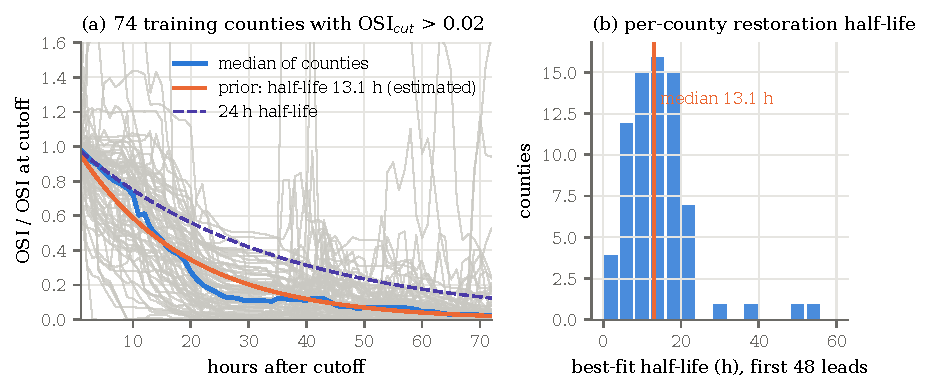
\includegraphics[width=.6\linewidth]{fig2_kinetics}
\caption{Restoration kinetics after the cutoff. (a) OSI relative to its cutoff value for the 74 training counties with $\osi_{\mathrm{cut}}>0.02$ (grey), their median, and the exponential prior with the estimated half-life versus a 24-h half-life. (b) Distribution of per-county best-fit half-lives.}\label{fig:kinetics}\end{figure}

\subsection{Two gradient-boosting members with one loss}
Both submitted members are LightGBM regressors \citep{ke2017} trained on the pooled county$\times$lead rows (191 counties $\times$ 143 leads $\approx$ 27{,}000 rows per outer fold) with the same 209 features and squared-error loss; they differ in target and capacity. Every county has weight 1. Reweighting by net inflow and cutoff OSI moved the loss off the official pooled RMSE and is not used.
\begin{itemize}
\item \textbf{Kinetics member} predicts the residual $S_c(\ell)-\hat S^{\,0}_c(\ell)$; its forecast is $\max(0,\hat S^{\,0}_c(\ell)+\text{residual})$. It is deliberately small (350 trees, learning rate 0.035, 15 leaves, depth 5, minimum 100 rows per leaf, 85\% column sampling, $L_2=10$).
\item \textbf{Direct member} predicts $S_c(\ell)$ itself with more capacity (800 trees, learning rate 0.02, 31 leaves, depth 5, minimum 60 rows per leaf, 80\% row and 50\% column subsampling, $L_2=10$). The decay curves are among its features (Fig.~\ref{fig:importance}b).
\end{itemize}
This is a \emph{direct} multi-step strategy \citep{bentaieb2012,taieb2016}---one model for all leads with $\ell$ as an input---rather than a recursive one, the right choice when no new observations arrive to correct a recursion.

\paragraph{Horizon-balanced loss.} The official score is the mean rank over four pooled RMSEs, each computed on cells $j\ge h$. With one shared trajectory, the average of the four horizon MSEs equals $\sum_j w_j\,e_j^2$ per county with
\begin{equation}
w_j=\tfrac14\sum_{h\in\{1,6,24,48\}}\frac{\mathbf 1[j\ge h]}{144-h},
\end{equation}
so we train both members with these exact per-lead sample weights ($w_0=0$; lead 0 is never scored). They favour late leads slightly, because each late hour is scored four times. Training the direct member without them changes its RMSE by $-0.2/+1.0/+2.6/+3.3\%$ at the four horizons.

\subsection{Lead-dependent convex stacking, and a member we removed}
The two submitted members are combined with non-negative weights that sum to one---Breiman's stacked regressions \citep{breiman1996}---fitted separately for three buckets of the forecast hour, $j\in[1,12]$, $[13,48]$ and $[49,143]$, by minimising the mean over horizons of the relative RMSE plus a quadratic pull of $0.01$ toward equal weights. The weights are fit on inner out-of-fold predictions. On the full development set they are 0.75/0.25, 0.48/0.52 and 0.00/1.00 (kinetics/direct): the prior's residual model carries the first hours, and the direct member carries the hours after 48.

A third member was trained to catch counties that are still rising at the cutoff. It used the kinetics residual target and the same small configuration, but only counties with cutoff OSI above 0.01 or positive net flow $N_t-R_t$. Its out-of-fold RMSE is $0.01178/0.01094/0.00931/0.00887$, worse than both submitted members at every horizon, so it is an ablation row only and is not in the nested stack. That stack, \texttt{predictions\_tree\_stack.csv}, scores $0.01106/0.01010/0.00824/0.00754$.

\subsection{A sequence-model view of the same information}\label{sec:seq}
The stack sees the record only through summaries we chose in advance. The sequence model reads the raw record: each county is one 216-step sequence with 36 channels---25 weather channels at every hour; $P_t$, $N_t$, $D_t$, $R_t$ and reconstructed OSI, rounded to four decimals and set to zero after the cutoff, with an observed-hour flag; hour-of-day sine and cosine; hours since the cutoff; log customers; and the prior of Eq.~(1) over the forecast hours. The network is a two-layer bidirectional selective state-space model \citep{gu2023mamba,gu2022s4,wang2025mamba}: width 24, state size 8, 22{,}201 parameters. A backward scan is legitimate because the sequence contains no post-cutoff outage information; the mutation test of Section~\ref{sec:data} is applied to these inputs too. Cross-validation and the final fit both use a severity-stratified 15\% county holdout for early stopping, so the cosine schedule is the same 120-epoch budget the cross-validation runs saw. Four seeds are averaged. The holdout is the protocol the cross-validation already validated; we do not refit a median epoch on all 239 counties under a shorter schedule.

The submitted trajectory is an equal half of the nested two-tree stack and the sequence model. The alternative is the same three lead buckets, with weights refit on four outer folds and scored on the fifth. Those cross-fitted sequence weights in hours 1--12 span 0.63--0.78 and the tree weights in hours 13--48 span 0.55--0.85, the pattern of weights fit to fold noise. The paired county bootstrap of that cross-fit against the half has improvement fractions 0.54/0.78/0.66/0.44, and every 95\% interval of the RMSE difference includes zero, including a positive mean difference at $t{+}48$\,h. The half is the file we submit. Its fold-held-out score, which needs no weight fit, is $0.01062/0.00967/0.00805/0.00710$. The cross-fit itself is $0.01061/0.00964/0.00803/0.00710$.

\subsection{Validation protocol}
Because test counties are unseen, validation holds out whole counties: five folds stratified by state$\times$\texttt{severity\_tier}, all 216 rows of a county in one fold \citep{bergmeir2012,roberts2017}; each held-out county is represented as a test county (72 observed hours plus weather). The two-tree stack in Table~\ref{tab:results} uses weights fitted on inner folds only. The submitted half does not fit a mixing weight. The lead-bucket row refits its weights with each outer fold held out. RMSEs are pooled over held-out county-hours before the square root, as in the official metric. Uncertainty uses a county-level bootstrap (2{,}000 resamples); model comparisons use a paired county bootstrap of the RMSE difference (3{,}000). Base seed 42 is combined with deterministic fold-specific offsets documented in the code; LightGBM runs in deterministic mode and PyTorch single-threaded with deterministic algorithms.

\section{Results}\label{sec:results}
\begin{table}[tb]\centering\footnotesize
\caption{Pooled out-of-fold RMSE by horizon, 239 training counties held out in five county-grouped folds (lower is better). Rel.\ = mean over horizons of RMSE relative to climatology. The bold row is the submitted equal half. The lead-bucket row refits mix weights with each fold held out and did not beat the half on the paired bootstrap.}\label{tab:results}
\begin{tabular}{@{}llrrrrr@{}}\toprule
 & Model & $t{+}1$\,h & $t{+}6$\,h & $t{+}24$\,h & $t{+}48$\,h & Rel.\\ \midrule
\multirow{4}{*}{\rotatebox{90}{\scriptsize baselines}}
 & Zero & 0.02349 & 0.01982 & 0.01209 & 0.00987 & 1.069\\
 & Mean trajectory of training counties (climatology) & 0.02165 & 0.01836 & 0.01137 & 0.00940 & 1.000\\
 & Persistence of the cutoff OSI & 0.06326 & 0.06419 & 0.06715 & 0.06921 & 4.921\\
 & Cutoff OSI with 24-h half-life & 0.01434 & 0.01367 & 0.01211 & 0.01059 & 0.900\\
\midrule
\multirow{6}{*}{\rotatebox{90}{\scriptsize ablations}}
 & Restoration prior alone ($H$ estimated) & 0.01306 & 0.01217 & 0.01022 & 0.00954 & 0.795\\
 & Weather/exposure/lead-only direct GBM & 0.01674 & 0.01423 & 0.00957 & 0.00765 & 0.801\\
 & Direct GBM, small configuration & 0.01251 & 0.01080 & 0.00855 & 0.00788 & 0.689\\
 & Direct GBM, no lead weights & 0.01209 & 0.01061 & 0.00842 & 0.00771 & 0.674\\
 & Kinetics GBM with fixed 24-h half-life & 0.01182 & 0.01091 & 0.00896 & 0.00804 & 0.696\\
 & Delayed-onset GBM (ablation only) & 0.01178 & 0.01094 & 0.00931 & 0.00887 & 0.725\\
\midrule
\multirow{3}{*}{\rotatebox{90}{\scriptsize trees}}
 & Kinetics GBM & 0.01127 & 0.01035 & 0.00850 & 0.00783 & 0.666\\
 & Direct GBM & 0.01212 & 0.01050 & 0.00820 & 0.00747 & 0.662\\
 & Two-tree stack, nested lead buckets & 0.01106 & 0.01010 & 0.00824 & 0.00754 & 0.647\\
\midrule
\multirow{3}{*}{\rotatebox{90}{\scriptsize final}}
 & Sequence model (four seeds) & 0.01096 & 0.00998 & 0.00849 & 0.00712 & 0.638\\
 & Lead-bucket blend, each fold held out & 0.01061 & 0.00964 & 0.00803 & 0.00710 & 0.619\\
 & \textbf{Equal half of stack and sequence (reported)} & \textbf{0.01062} & \textbf{0.00967} & \textbf{0.00805} & \textbf{0.00710} & \textbf{0.620}\\
\bottomrule
\end{tabular}\end{table}

Table~\ref{tab:results} is the ablation ladder for this run. The restoration prior alone still removes 40\% of the climatology error at $t{+}1$\,h ($0.01306$ against $0.02165$). The estimated half-life beats a fixed 24\,h half-life at every horizon. The weather/exposure/lead ablation excludes the neighbour cutoff-OSI features. The delayed-onset member does not help: it is worse than kinetics and direct at all four horizons, and it is not in the stack.

The sequence model, at $0.01096/0.00998/0.00849/0.00712$, is the best single model. The equal half is better than the stack by 4.0/4.2/2.3/5.9\% and better than the sequence model by 3.1/3.1/5.2/0.4\%. Relative to climatology that is a 51/47/29/25\% reduction. A paired county bootstrap gives P(better) fractions 0.95/0.96/0.80/0.99 against the stack and 0.76/0.76/0.90/0.59 against the sequence model. Only the $t{+}48$\,h comparison with the stack has a 95\% interval entirely below zero; the other seven intervals include zero. The two members' errors correlate at 0.86, so the average is a variance reduction rather than a hand-off between uncorrelated experts. Across folds the half is worse than the stack in 3 of 20 fold-horizon cells, and one of those cells (one fold, $t{+}24$\,h) is 10\% worse. The lead-bucket cross-fit is within a few ten-thousandths of the half and does not win the same paired test, which is why it is not the submitted file \citep{breiman1996,makridakis2022}.

\begin{figure}[tb]\centering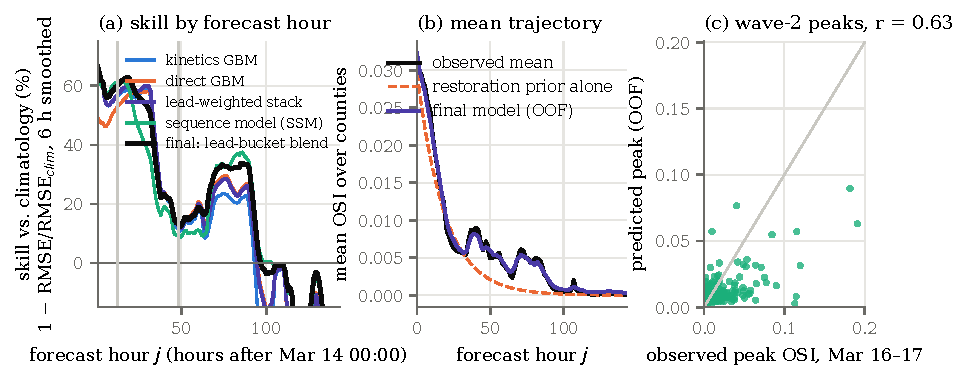
\includegraphics[width=.75\linewidth]{fig3_skill}
\caption{Out-of-fold skill of the submitted equal half. (a) Skill relative to climatology by forecast hour (vertical lines: the bucket boundaries used by the tree stack). (b) Mean predicted and observed trajectories; the prior captures restoration but not the second wave. (c) Second-wave county peaks, observed versus predicted.}\label{fig:skill}\end{figure}

\section{Discussion}\label{sec:discussion}
\paragraph{Where the error is.} In the $t{+}1$\,h window, March 14 holds 78\% of the target energy and 52\% of the submitted blend's squared error; March 16--17 holds 11\% of the energy but 25\% of the error. Forest County, PA (FIPS 42053) alone holds 28\%. Its OSI was 0.09 and still rising at the cutoff (net inflow $N_t-R_t>0$) and peaked at 0.545 six hours later; the out-of-fold prediction of the submitted blend peaks at 0.14 (Fig.~\ref{fig:cases}, left). Ten of the 74 substantially affected training counties keep rising after the cutoff; six have positive net inflow at the cutoff, against one in five of the other affected counties, so a signal exists, and the onset member was built to use it. Ten cases are too few: that member was worse at every horizon, and squared error still shrinks extremes. Over all cells with observed OSI above 0.05 the blend predicts 81\% of the observed value on average. Under RMSE that shrinkage is the right trade-off for the population, and it remains the largest identifiable weakness. Morrow County, OH (centre) is the typical case, a deep first-wave outage restored along the prior; Clay County, WV (right) is the second wave, where the weather path anticipates the rise and the peak is still low. The ten counties with the largest squared error account for 61\%.

\begin{figure}[tb]\centering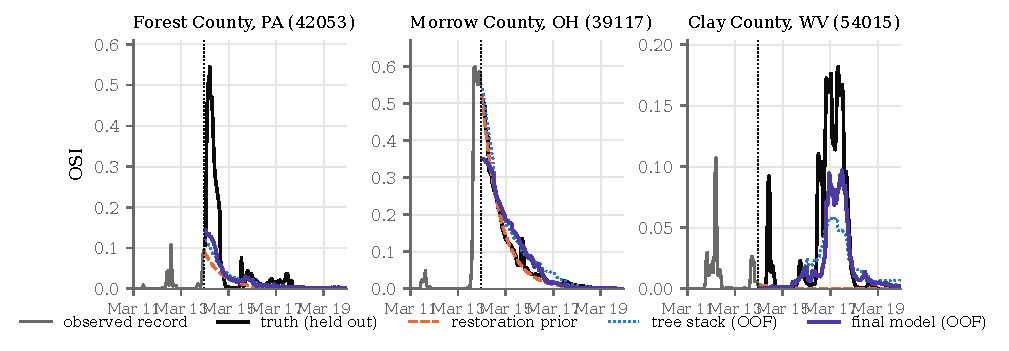
\includegraphics[width=.66\linewidth]{fig4_cases}
\caption{Held-out trajectories for three training counties. Grey: the record the models were allowed to see; black: the withheld truth; dashed: the restoration prior; purple: the submitted equal half.}\label{fig:cases}\end{figure}

\paragraph{Why the second wave is harder.} Across training counties, with wave 1 taken as March 13--15 and wave 2 as March 16--19 (\texttt{shape\_diagnostics.py}), the peak gust of the first wave explains outage peaks reasonably well (Pearson $r=0.41$ between peak gust and peak OSI), but for the second wave the same correlation is $-0.08$, and second-wave peaks are only weakly related to first-wave peaks ($r=0.15$). Two mechanisms are consistent with this: vegetation and equipment that fail in the first event are no longer there to fail in the second, and crews and mutual-assistance resources are already positioned \citep{guikema2014,wanik2015}. The data cannot separate the two; what a model can exploit is the interaction between the fragility revealed by the first wave and the second-wave winds. In the kinetics member, weather accounts for 60\% of split gain and observed outage history a further 26\% (Fig.~\ref{fig:importance}a). March 16--17 RMSE is 27\% below climatology, and for the tree stack alone: 22\%. Second-wave peaks correlate at 0.63 with the submitted predictions.

\begin{figure}[tb]\centering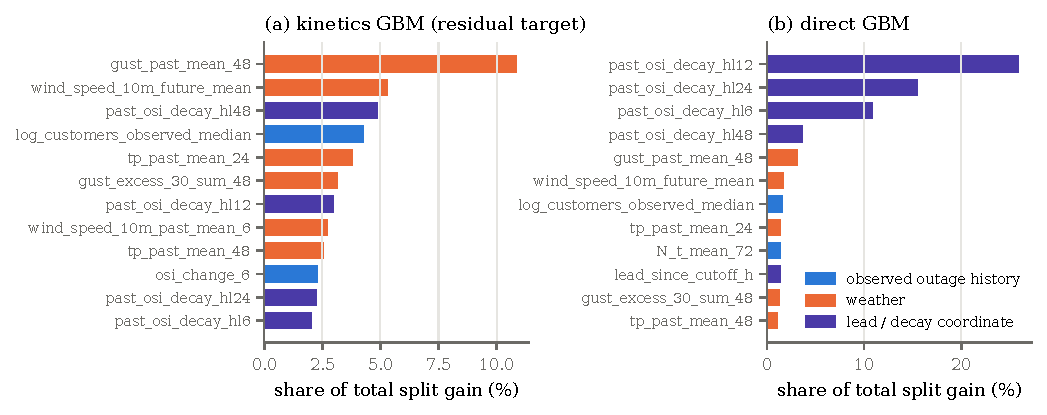
\includegraphics[width=.44\linewidth]{fig5_importance}
\caption{Top-12 features by share of split gain, averaged over the five outer folds. Once the decay is removed (a), the residual is explained mainly by weather history and the observed outage state; the direct member (b) spends most of its gain reconstructing the decay.}\label{fig:importance}\end{figure}

\paragraph{What did not help.} The delayed-onset member is the negative result from this round: same features, same residual target, trained only on the counties the Forest County pattern belongs to, and worse at every horizon, so it is not in \texttt{predictions.csv}. On this 209-feature panel, a hurdle model \citep{cragg1971} stayed within 1\% of the direct member, Tweedie and $\log(1+100y)$ targets were worse, five-seed averaging of the direct member moved RMSE by at most 0.61\%, and an analogue ensemble \citep{dellemonache2013} raised RMSE by 39.0/38.0/23.2/17.6\% at the four horizons. The addition that survived is the sequence model, because it reads the hourly record rather than the fixed summaries \citep{makridakis2022,nateghi2014}.

\paragraph{Reproducibility.} The archive rebuilds \texttt{predictions.csv} from the three organiser files in \texttt{data/}; those files are not in the repository. Unpacking this code and installing the pinned requirements into a fresh prefix (CPython 3.13.11, macOS 26.6 arm64, torch 2.14.0, LightGBM 4.6.0) reproduced \texttt{predictions.csv} and \texttt{predictions\_tree\_stack.csv} byte for byte. The sequence model uses the early-stopping holdout in every fit. PyTorch can differ in the last decimals on another CPU. Windows is unverified.

\section{Limitations and conclusions}\label{sec:conclusion}
The evidence comes from one storm sequence in one region; the half-life and the tree-stack bucket weights are properties of this event and should be re-estimated for another. Weather is reanalysis, not an operational forecast, so the scores are optimistic for real-time use. Folds are stratified but not spatially blocked, so mild optimism from correlated neighbours cannot be excluded. The submitted score is the equal half, which does not fit a mixing weight on the counties it is scored on. The sequence model is less transparent than the stack, four seeds are still few, and its cross-platform bit-reproducibility is weaker. The model produces point forecasts; a utility pre-positioning crews would want quantiles. The covariates we would add next are tree canopy, line miles and rural--urban class \citep{cerrai2019,wanik2015}.

The submitted file is one trajectory per county: a restoration prior, residual boosting for departures from it, a direct level model, and a sequence reading of the same record, averaged with equal weight. The onset specialist was the test of whether the Forest County pattern could be learned as its own member, and it could not. On held-out counties the reported blend removes 51\% of climatology RMSE at $t{+}1$\,h and 25\% at $t{+}48$\,h.

\clearpage
\small
\bibliographystyle{unsrtnat}
\begin{thebibliography}{23}
\bibitem[Ye et al.(2025)]{ye2025sarimax} H.~Ye, Q.~Sun, and Y.~Yang. SARIMAX-based power outage prediction during extreme weather events. \emph{arXiv:2511.01017}, 2025. Fourth place, 2025 INFORMS DMS Data Challenge.
\bibitem[Cerrai et al.(2019)]{cerrai2019} D.~Cerrai, D.~W. Wanik, M.~A.~E. Bhuiyan, X.~Zhang, J.~Yang, M.~E.~B. Frediani, and E.~N. Anagnostou. Predicting storm outages through new representations of weather and vegetation. \emph{IEEE Access}, 7:29639--29654, 2019.
\bibitem[Liu et al.(2007)]{liu2007} H.~Liu, R.~A. Davidson, and T.~V. Apanasovich. Statistical forecasting of electric power restoration times in hurricanes and ice storms. \emph{IEEE Transactions on Power Systems}, 22(4):2270--2279, 2007.
\bibitem[Nateghi et al.(2011)]{nateghi2011} R.~Nateghi, S.~D. Guikema, and S.~M. Quiring. Comparison and validation of statistical methods for predicting power outage durations in the event of hurricanes. \emph{Risk Analysis}, 31(12):1897--1906, 2011.
\bibitem[Ke et al.(2017)]{ke2017} G.~Ke, Q.~Meng, T.~Finley, T.~Wang, W.~Chen, W.~Ma, Q.~Ye, and T.-Y. Liu. LightGBM: A highly efficient gradient boosting decision tree. In \emph{Advances in Neural Information Processing Systems 30}, pages 3146--3154, 2017.
\bibitem[Ben Taieb et al.(2012)]{bentaieb2012} S.~Ben Taieb, G.~Bontempi, A.~F. Atiya, and A.~Sorjamaa. A review and comparison of strategies for multi-step ahead time series forecasting based on the NN5 forecasting competition. \emph{Expert Systems with Applications}, 39(8):7067--7083, 2012.
\bibitem[Taieb and Atiya(2016)]{taieb2016} S.~B. Taieb and A.~F. Atiya. A bias and variance analysis for multistep-ahead time series forecasting. \emph{IEEE Transactions on Neural Networks and Learning Systems}, 27(1):62--76, 2016.
\bibitem[Breiman(1996)]{breiman1996} L.~Breiman. Stacked regressions. \emph{Machine Learning}, 24(1):49--64, 1996.
\bibitem[Bergmeir and Ben\'itez(2012)]{bergmeir2012} C.~Bergmeir and J.~M. Ben\'itez. On the use of cross-validation for time series predictor evaluation. \emph{Information Sciences}, 191:192--213, 2012.
\bibitem[Roberts et al.(2017)]{roberts2017} D.~R. Roberts, V.~Bahn, S.~Ciuti, M.~S. Boyce, J.~Elith, G.~Guillera-Arroita, S.~Hauenstein, J.~J. Lahoz-Monfort, B.~Schr\"oder, W.~Thuiller, D.~I. Warton, B.~A. Wintle, F.~Hartig, and C.~F. Dormann. Cross-validation strategies for data with temporal, spatial, hierarchical, or phylogenetic structure. \emph{Ecography}, 40(8):913--929, 2017.
\bibitem[Guikema et al.(2014)]{guikema2014} S.~D. Guikema, R.~Nateghi, S.~M. Quiring, A.~Staid, A.~C. Reilly, and M.~Gao. Predicting hurricane power outages to support storm response planning. \emph{IEEE Access}, 2:1364--1373, 2014.
\bibitem[Wanik et al.(2015)]{wanik2015} D.~W. Wanik, E.~N. Anagnostou, B.~M. Hartman, M.~E.~B. Frediani, and M.~Astitha. Storm outage modeling for an electric distribution network in Northeastern USA. \emph{Natural Hazards}, 79(2):1359--1384, 2015.
\bibitem[Cragg(1971)]{cragg1971} J.~G. Cragg. Some statistical models for limited dependent variables with application to the demand for durable goods. \emph{Econometrica}, 39(5):829--844, 1971.
\bibitem[Geurts et al.(2006)]{geurts2006} P.~Geurts, D.~Ernst, and L.~Wehenkel. Extremely randomized trees. \emph{Machine Learning}, 63(1):3--42, 2006.
\bibitem[Delle Monache et al.(2013)]{dellemonache2013} L.~Delle Monache, F.~A. Eckel, D.~L. Rife, B.~Nagarajan, and K.~Searight. Probabilistic weather prediction with an analog ensemble. \emph{Monthly Weather Review}, 141(10):3498--3516, 2013.
\bibitem[Makridakis et al.(2022)]{makridakis2022} S.~Makridakis, E.~Spiliotis, and V.~Assimakopoulos. M5 accuracy competition: Results, findings, and conclusions. \emph{International Journal of Forecasting}, 38(4):1346--1364, 2022.
\bibitem[Nateghi et al.(2014)]{nateghi2014} R.~Nateghi, S.~D. Guikema, and S.~M. Quiring. Power outage estimation for tropical cyclones: Improved accuracy with simpler models. \emph{Risk Analysis}, 34(6):1069--1078, 2014.
\bibitem[Fatima et al.(2024)]{fatima2024} K.~Fatima, H.~Shareef, F.~Costa, A.~Bajwa, and L.~Wong. Machine learning for power outage prediction during hurricanes: An extensive review. \emph{Engineering Applications of Artificial Intelligence}, 133:108056, 2024.
\bibitem[Hersbach et al.(2020)]{hersbach2020} H.~Hersbach, B.~Bell, P.~Berrisford, S.~Hirahara, A.~Hor\'anyi, J.~Mu\~noz-Sabater, et al. The ERA5 global reanalysis. \emph{Quarterly Journal of the Royal Meteorological Society}, 146(730):1999--2049, 2020.
\bibitem[De Pondeca et al.(2011)]{depondeca2011} M.~S.~F.~V. De Pondeca, G.~S. Manikin, G.~DiMego, S.~G. Benjamin, D.~F. Parrish, R.~J. Purser, et al. The Real-Time Mesoscale Analysis at NOAA's National Centers for Environmental Prediction: Current status and development. \emph{Weather and Forecasting}, 26(5):593--612, 2011.
\bibitem[Gu and Dao(2023)]{gu2023mamba} A.~Gu and T.~Dao. Mamba: Linear-time sequence modeling with selective state spaces. \emph{arXiv:2312.00752}, 2023.
\bibitem[Gu et al.(2022)]{gu2022s4} A.~Gu, K.~Goel, and C.~R\'e. Efficiently modeling long sequences with structured state spaces. In \emph{International Conference on Learning Representations (ICLR)}, 2022.
\bibitem[Wang et al.(2025)]{wang2025mamba} Z.~Wang, F.~Kong, S.~Feng, M.~Wang, X.~Yang, H.~Zhao, D.~Wang, and Y.~Zhang. Is Mamba effective for time series forecasting? \emph{Neurocomputing}, 619:129178, 2025.
\end{thebibliography}
\end{document}
